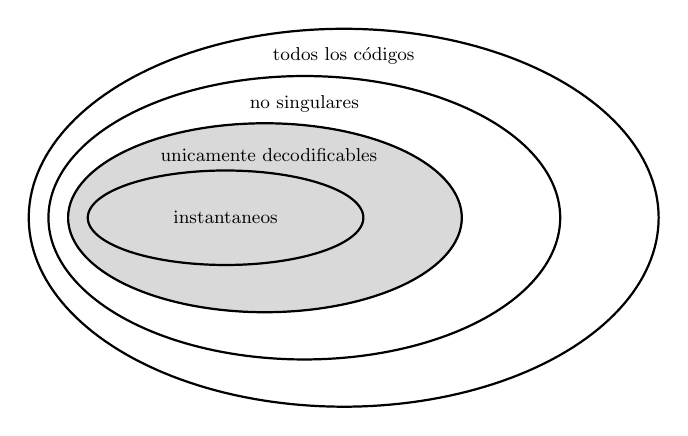
\begin{tikzpicture}
\shorthandoff{>}
\filldraw[fill=gray!30,domain=0:360, samples=200] plot ({2.5*cos(\x)+.5},{1.2*sin(\x)});
%%%%
\draw[thick,domain=0:360, samples=200] plot ({1.75*cos(\x)},{.6*sin(\x)});
\draw (0,0) node[scale=.75] {\small instantaneos};
%
\draw[thick,domain=0:360, samples=200] plot ({2.5*cos(\x)+.5},{1.2*sin(\x)});
\draw (.55,.8) node[scale=.75] {\small  unicamente decodificables};
%
\draw[thick,domain=0:360, samples=200] plot ({3.25*cos(\x)+1},{1.8*sin(\x)});
\draw (1,1.45) node[scale=.75] {\small no singulares};
%
\draw[thick,domain=0:360, samples=200] plot ({4*cos(\x)+1.5},{2.4*sin(\x)});
\draw (1.5,2.05) node[scale=.75] {\small todos los c\'odigos};
\end{tikzpicture}
